\section{Centering and Scaling}\label{sec:centerScale}
%
As previously defined, the general (linear or non-linear) low-dimensional state representation for the conserved and target states are defined, respectively, as
%
\begin{align}
	\consVecRom &\defEq \consVecCent + \consScale \nnLayer_{\decoderVar,\consVar}\left(\consVecCoef\right), \\
	\primVecRom &\defEq \primVecCent + \primScale \nnLayer_{\decoderVar,\primVar} \left(\primVecCoef\right),
\end{align}
%
where, again, the functions $\nnLayer_{\decoderVar,\consVar}\left(\consVecCoef\right) = \consTrial \consVecCoef$ and $\nnLayer_{\decoderVar,\primVar}\left(\primVecCoef\right) = \primTrial \primVecCoef$ for a linear trial space. This decomposition by centering ($\consVecCent$, $\primVecCent$) and the scaling ($\consScale$, $\primScale$) operation is often referred to as \textit{feature scaling} in the machine learning community, whereby the training datasets are constructed (as noted in Eqs~\ref{eq:consSnapMat} and~\ref{eq:primSnapMat}) by
%
\begin{align}
	\consDataMatUns &= \left[ \consScaleInv\left[\consFunc{\initTime} - \consVecCent\right], \; \hdots \; , \; \consScaleInv\left[\consFunc{\finalTime} - \consVecCent \right] \right], \\
	\primDataMatUns &= \left[ \primScaleInv\left[\primFunc{\initTime} - \consVecCent\right], \; \hdots \; , \; \primScaleInv\left[\primFunc{\finalTime} - \primVecCent \right] \right].
\end{align}
%
The choice of $\consVecCent$/$\consScale$ and $\primVecCent$/$\primScale$ has a measurable influence on the accuracy of the above approximations, particularly for variables of extremely disparate magnitudes. Before demonstrating this fact, several popular methods of centering and scaling are outlined and compared.

\paragraph*{Centering}\mbox{}\\
%
With the exception of centering for min-max scaling, all centering methods described here are considered to be spatially-variant, i.e. $\consVecCent \defEq \consVecCent(\spatialVec)$, $\primVecCent \defEq \primVecCent(\spatialVec)$. Each is described in turn.

\begin{enumerate}
	\item \textit{Initial condition}: Centering about the initial condition, i.e. $\consVecCent = \consVec(\initTime)$ or $\primVecCent = \primVec(\initTime)$, results in approximation of the unsteady state as perturbations about the initial condition. In the case of a linear trial space, this guarantees exact satisfaction of the initial conditions, as the projection of the zero vector (the initial condition subtracted by itself) is identically zero. In the case of autoencoder non-linear manifold methods, however, this is merely satisfied approximately, and near-satisfaction is encouraged by including the zero vector in the training set and initializing the non-linear manifold PROM from the encoding of the zero vector, as in~\cite{Lee2020}.

	\item \textit{Mean}: The mean field centering computes the centering vector as the arithmetic mean of the data snapshots,
	%
	\begin{align}
		\consVecCent &= \frac{1}{\numSnaps} \sum_{\timeIdx=1}^{\numSnaps} \consVec^{\timeIdx} \label{eq:meanCentCons}\\
		\primVecCent &= \frac{1}{\numSnaps} \sum_{\timeIdx=1}^{\numSnaps} \primVec^{\timeIdx} \label{eq:meanCentPrim}
	\end{align}
	%
	This concept is fairly common in the turbulence modeling community, which often seeks to accurately describe unsteady perturbations about the time-averaged field for statistically-stationary flows. In the same sense, centering data snapshots about the mean field ensures that the low-dimensional representation accurately captures these small-scale fluctuations which would otherwise be dwarfed by the mean field.

\end{enumerate}

\paragraph*{Scaling}\mbox{}\\
%
For all methods described below, the scaling matrices $\consScale$, $\primScale$ are composed of constant scalars which are specific to a given state variable (e.g., density, velocity) but are not specific to spatial location. This can be written as as
%
\begin{align}
	\consScale &\defEq diag\left(\consScaleVecVar{1}^\top, \; \hdots, \; \consScaleVecVar{\numVars}^\top \right), \quad \consScaleVecVar{\varIdx}\left(\spatialVec_{\dummyIdx}\right) = \consScaleVar{\varIdx} \; \forall \; \dummyIdx \in \{1, \; \hdots, \; \numCells\} \\
	\primScale &\defEq diag\left(\primScaleVecVar{1}^\top, \; \hdots, \; \primScaleVecVar{\numVars}^\top \right), \quad \primScaleVecVar{\varIdx}\left(\spatialVec_{\dummyIdx}\right) = \primScaleVar{\varIdx} \; \forall \; \dummyIdx \in \{1, \; \hdots, \; \numCells\}
\end{align}
%
where $\consScaleVecVar{\varIdx}$, $\primScaleVecVar{\varIdx} \in \mathbb{R}$ is the constant conservative/target scaling value for the $\varIdx$ state variable.

\begin{enumerate}
	\item $\ell^2$\textit{-norm}: Scaling by the $\ell^2$-norm method is motivated by that proposed by Lumley and Poje~\cite{Lumley1997}, and is computed as
	%
	\begin{align}
		\consScaleVar{\varIdx} &= \frac{1}{\numSnaps \numCells} \sum_{\timeIdx=1}^{\numSnaps} \left\Vert \consVecVar^{\timeIdx} - \consVecCentVar \right\Vert^2 \\
		\primScaleVar{\varIdx} &= \frac{1}{\numSnaps \numCells} \sum_{\timeIdx=1}^{\numSnaps} \left\Vert \primVecVar^{\timeIdx} - \primVecCentVar \right\Vert^2
	\end{align}
	This has the effect of ensuring that all state variable vectors have a length (in the Euclidean norm) close to unity. This is closely related to the POD, which computes the distance between the data and their projection in the $\ell^2$ norm.

	\item \textit{Min-max}: Min-max feature scaling, composed of associated centering and scaling operations, has the effect of ensuring that all values in the modified dataset fall in the range $[0.0, \; 1.0]$. For the $\varIdx$th state variable (e.g. density, velocity), the centering vector is computed as
	%
	\begin{align}
		\consValCentVar &= min\left(\consDataMatVar\right), \quad \consVecCentVar\left(\spatialVec_{\dummyIdx}\right) = \consValCentVar \; \forall \; \dummyIdx \in \{1, \; \hdots, \; \numCells\} \\
		\primValCentVar &= min\left(\primDataMatVar\right), \quad \primVecCentVar\left(\spatialVec_{\dummyIdx}\right) = \primValCentVar \; \forall \; \dummyIdx \in \{1, \; \hdots, \; \numCells\}
	\end{align}
	%
	where the data snapshot matrix for the $\varIdx$th state variable is given by
	%
	\begin{align}
		\consDataMatVar &\defEq \left[ \consVecVar\left(\initTime\right), \; \hdots, \; \consVecVar\left(\finalTime\right) \right] \label{eq:consDataMat}\\
		\primDataMatVar &\defEq \left[ \primVecVar\left(\initTime\right), \; \hdots, \; \primVecVar\left(\finalTime\right) \right] \label{eq:primDataMat}
	\end{align}
	%
	The scaling values are then computed as
	%
	\begin{align}
		\consScaleVar{\varIdx} &= max\left(\consDataMatVar\right) - min\left(\consDataMatVar\right) \\
		\primScaleVar{\varIdx} &= max\left(\primDataMatVar\right) - min\left(\primDataMatVar\right)
	\end{align}
	%
	where the data matrices are given as in Eqs.~\ref{eq:consDataMat} and~\ref{eq:primDataMat}. Note that this min-max scaling can be applied on top of an alternative centering method, e.g. centering by the initial condition and then min-max scaling. Such an operation for the conservative state would take the form
	%
	\begin{equation}
		\consVecVarUns = \frac{\consVecVar - \consVecCent - min\left(\consDataMatVar\right)}{max\left(\consDataMatVar\right) - min\left(\consDataMatVar\right)}
	\end{equation}
	%
	As such, min-max scaling will be referred to exclusively as a scaling operation which can be combined with a given centering method, or applied without alternative centering.
	
	Although min-max scaling is fairly common within the machine learning community, and is a simple method of ensuring that the data are roughly the same order of magnitude, this scaling has the effect of emphasizing outliers which define the maximum and minimum bounds of the state variables.
\end{enumerate}

\begin{figure}
	\begin{minipage}{0.32\linewidth}
		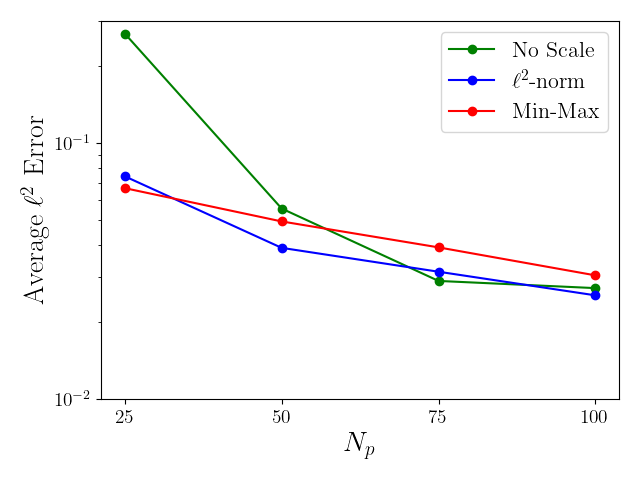
\includegraphics[width=0.99\linewidth]{Chapters/BestPractices/Images/errVsModes_centScale_centNone_Average_errorRaw.png}
		\subcaption{No centering.}
	\end{minipage}
	\begin{minipage}{0.32\linewidth}
		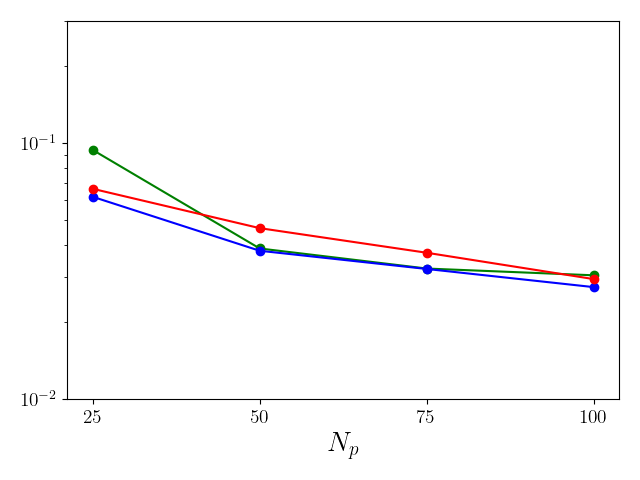
\includegraphics[width=0.99\linewidth]{Chapters/BestPractices/Images/errVsModes_centScale_centIC_Average_errorRaw.png}
		\subcaption{Initial condition.}
	\end{minipage}
	\begin{minipage}{0.32\linewidth}
		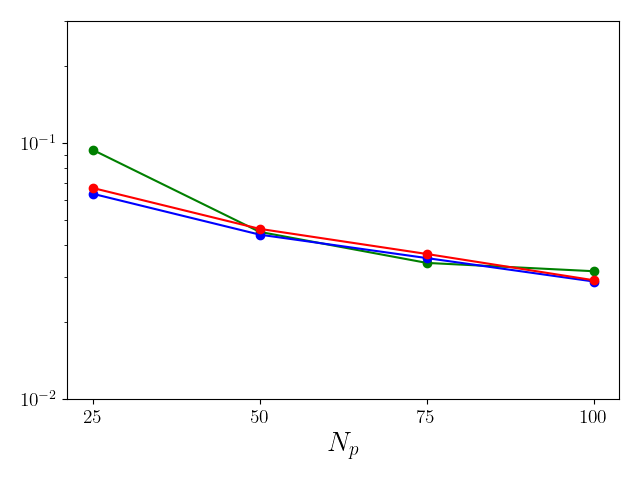
\includegraphics[width=0.99\linewidth]{Chapters/BestPractices/Images/errVsModes_centScale_centMean_Average_errorRaw.png}
		\subcaption{Time average.}
	\end{minipage}
	\caption{\label{fig:centScaleError}CVRC unsampled MP-LSVT PROM time-average error, $\numPrimModes = 25$, various trial space centerings.}
\end{figure}

\begin{figure}
	\begin{minipage}{0.49\linewidth}
		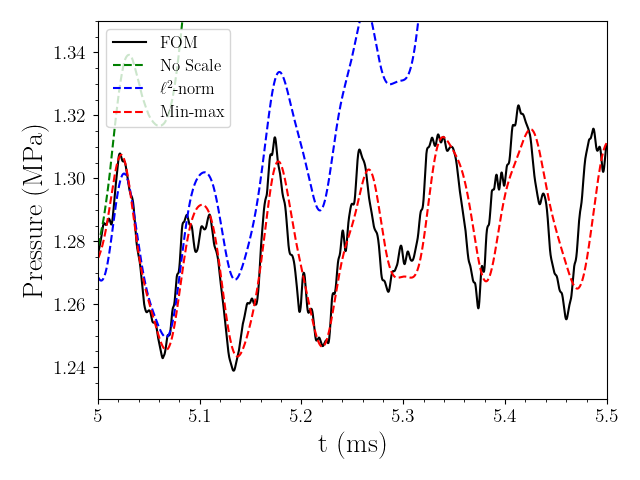
\includegraphics[width=0.99\linewidth]{Chapters/BestPractices/Images/pressure_probe_centScale_centNone.png}
		\subcaption{No centering.}
	\end{minipage}
	\begin{minipage}{0.49\linewidth}
		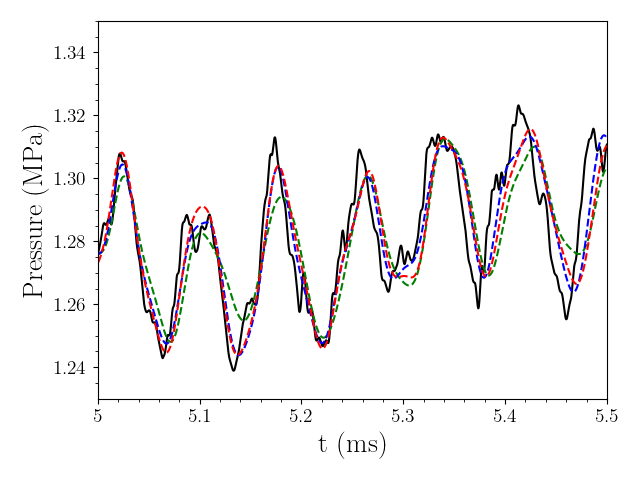
\includegraphics[width=0.99\linewidth]{Chapters/BestPractices/Images/pressure_probe_centScale_centIC.png}
		\subcaption{Initial condition.}
	\end{minipage}
	
	\centering
	\begin{minipage}{0.49\linewidth}
		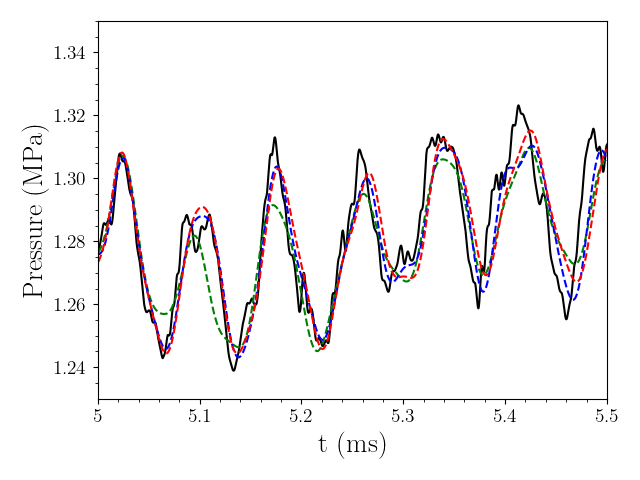
\includegraphics[width=0.99\linewidth]{Chapters/BestPractices/Images/pressure_probe_centScale_centMean.png}
		\subcaption{Time average.}
	\end{minipage}
	\caption{\label{fig:centScaleProbes}CVRC unsampled MP-LSVT PROM pressure probes, $\numPrimModes = 25$, various trial space centerings.}
\end{figure}

Time-average error results for the MP-LSVT PROMs of the truncated CVRC, for $\numPrimModes = \{25,\; 50,\; 75,\; 100\}$, are shown in Fig.~\ref{fig:centScaleError}, along with indicative pressure probe measurements in Fig.~\ref{fig:centScaleProbes}. Both instances in which centering is applied (either initial condition or time-average field) perform similarly, and scaling the state appears to improve the solution over cases without scaling. If no centering, however, the PROM accuracy is rather poor even in cases where scaling is also applied. 